\documentclass[]{IEEEtran}
\usepackage[utf8]{inputenc}
\usepackage[spanish,es-tabla]{babel}
\usepackage{amsmath}
\usepackage{amsfonts}
\usepackage{amssymb}
\usepackage{graphicx}
\usepackage{cite}
\usepackage{hyperref}

\title{Procesamiento de imágenes utilizando Deep learning y Carla 
Simulator}
\author{ 
Gatica, Isais \\ \small{email: isaiasgatica1@gmail.com} \\ \and 
Saez, Lautaro Andres \\ \small{email: lautaroandressaez@gmail.com } }
\date{}

\begin{document}
    \maketitle

    \begin{abstract}
        En este informe se presenta la implementación de una red Pix2Pix capaz de pasar de una imagen RGB a 
        una imagen segmentada donde cada color indica un objeto diferente. Se comenzara desde cero obteniendo el 
        dataset mediante el simulador CARLA para luego poder entrenar la red con una gran variedad de imagenes con 
        diferente clima y vegetación. Finalmente se probara con imagenes reales para analizar la viavilidad de entrenar una 
        red con un simulador y luego ingresarla en el mundo real.
    \end{abstract}

    \section{Introducción}

    En los ultimos años, debido a la necesidad de resolver cada vez mas complejos y la posibilidad de utilizar GPU's las redes neuronales han cobrado 
    gran importancia en nuetras vidas, y ya son parte del dia a dia, cosas tan simples como los filtros de Instagram basan 
    su reconocimiento facial en redes neuronales. 

    Las redes permiten resolver problemas que van desde la clasificación de imagenes hasta la conducción autonoma, claro esta 
    que para esto existen diferentes arquitecturas las cuales son expecificas para determinadas tareas, como el procesamiento de imagenes (CNN, GAN, YOLO), 
    procesamiento de texto (RNN), procesamiento de datos (NN).

    La desventaja principal de estos modelos supervisados es la necesidad de una dataset muy bien estructurado y para el cual es necesario 
    el trabajo humano, esta es la tarea mas importante y que si esta mal realizada el red no tendra un desempeño correcto.



    \section{Marco Teoríco}

    En esta sección se hara un breve marco teoríco de los conceptos basicos que se utilizaran en 
    el proyecto.

    \subsection{Deep Learning}

    Las redes neuronal son muy utilizadas en el campo de la minería de datos, debido a 
    su gran versatilidad. Dentro de este mundo existen 2 grandes tipos de entrenamientos 
    para los supervisados que dada una entrada $X$ se conoce la salida deseada $Y$ y 
    otros casos los algoritmos no supervisados como los modelos de Q-learning o los mapas autoorganizados (SOM).
    En este proyecto se opto por un entrenamiento supervisado.

    

    Para el modelado de la red neuronal se utilizó un modelo llamado Pix2Pix \cite{Pix2Pix}.
    El cual pertime dada una imagen de entrada $X$ obtener una imagen de salida $Y$.

    Este modelo consta de $2$ redes separadas, la primera se denominada el generador Fig.\ref{fig:generator}
    el cual deberá aprender a segmentar la imagen semanticamente. Y la segunda se llama el discriminador Fig.\ref{fig:discr}
    este se encarga de correguir al generador aprendiendo cuando una salida es "realista". 
    Llamaremos salida "realista" a aquella imagen que cumpla el objetivo esperado, en este caso sería una imagen segmentada 
    de coherente.
    
    \begin{figure}
        \centering
        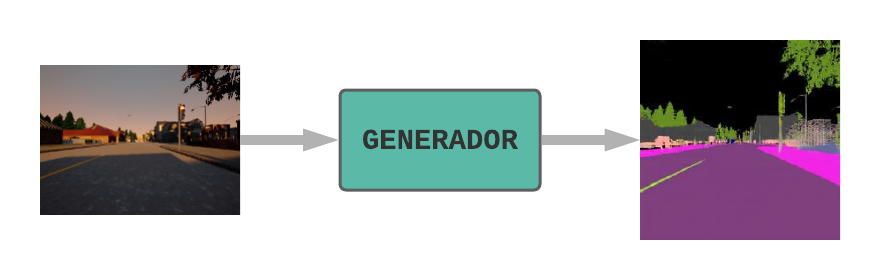
\includegraphics[width=.4\textwidth]{Imgs/Generador.png}
        \caption{Esquema de la red generativa.}
        \label{fig:generator}
    \end{figure}

    \begin{figure}
        \centering
        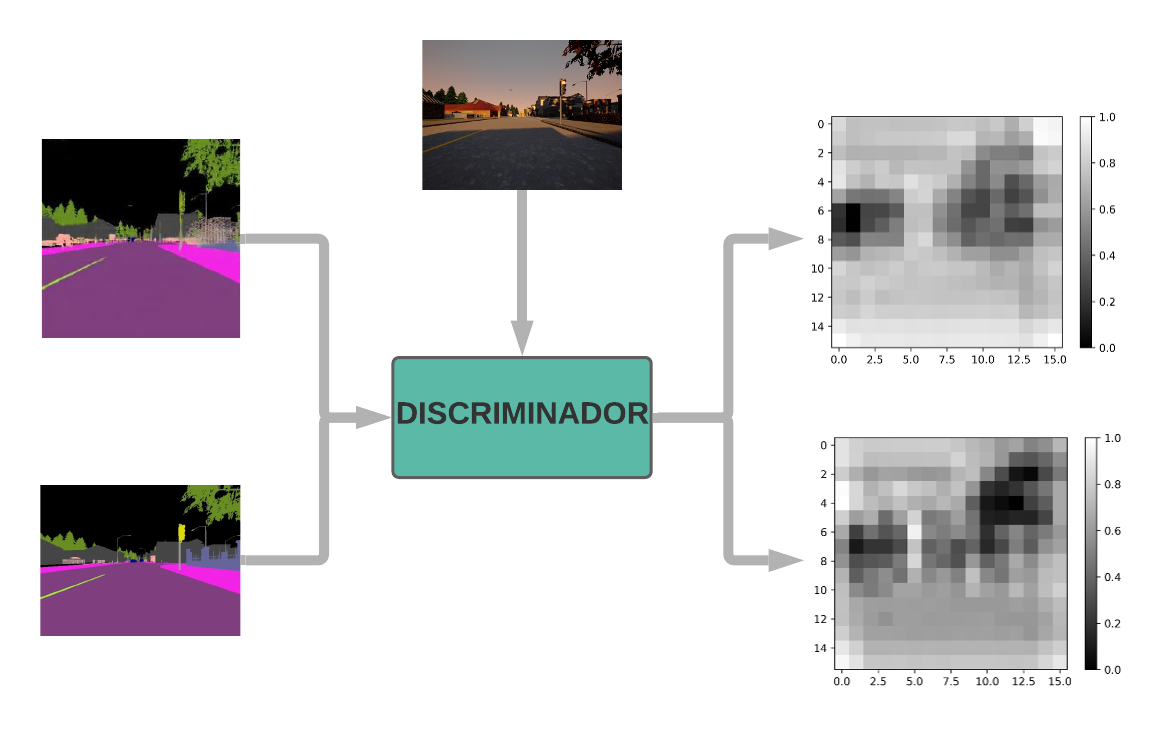
\includegraphics[width=.4\textwidth]{Imgs/Discriminador.png}
        \caption{Esquema de la red discriminativa.}
        \label{fig:discr}
    \end{figure}
    


    \subsubsection{Generador}

    El generador cuenta con una arquitetura denomina U-net \cite{U-Net}, la cual tiene 
    la cual posee una muy buena eficiencia debido a los bypass que existen entra las capas de convolución y 
    las capas de deconvulición. Con la finalidad de comprender de forma mas sencilla se puede observar 
    en la Fig.\ref{fig:u-net} dicha arquitectura.

    \begin{figure}
        \centering
        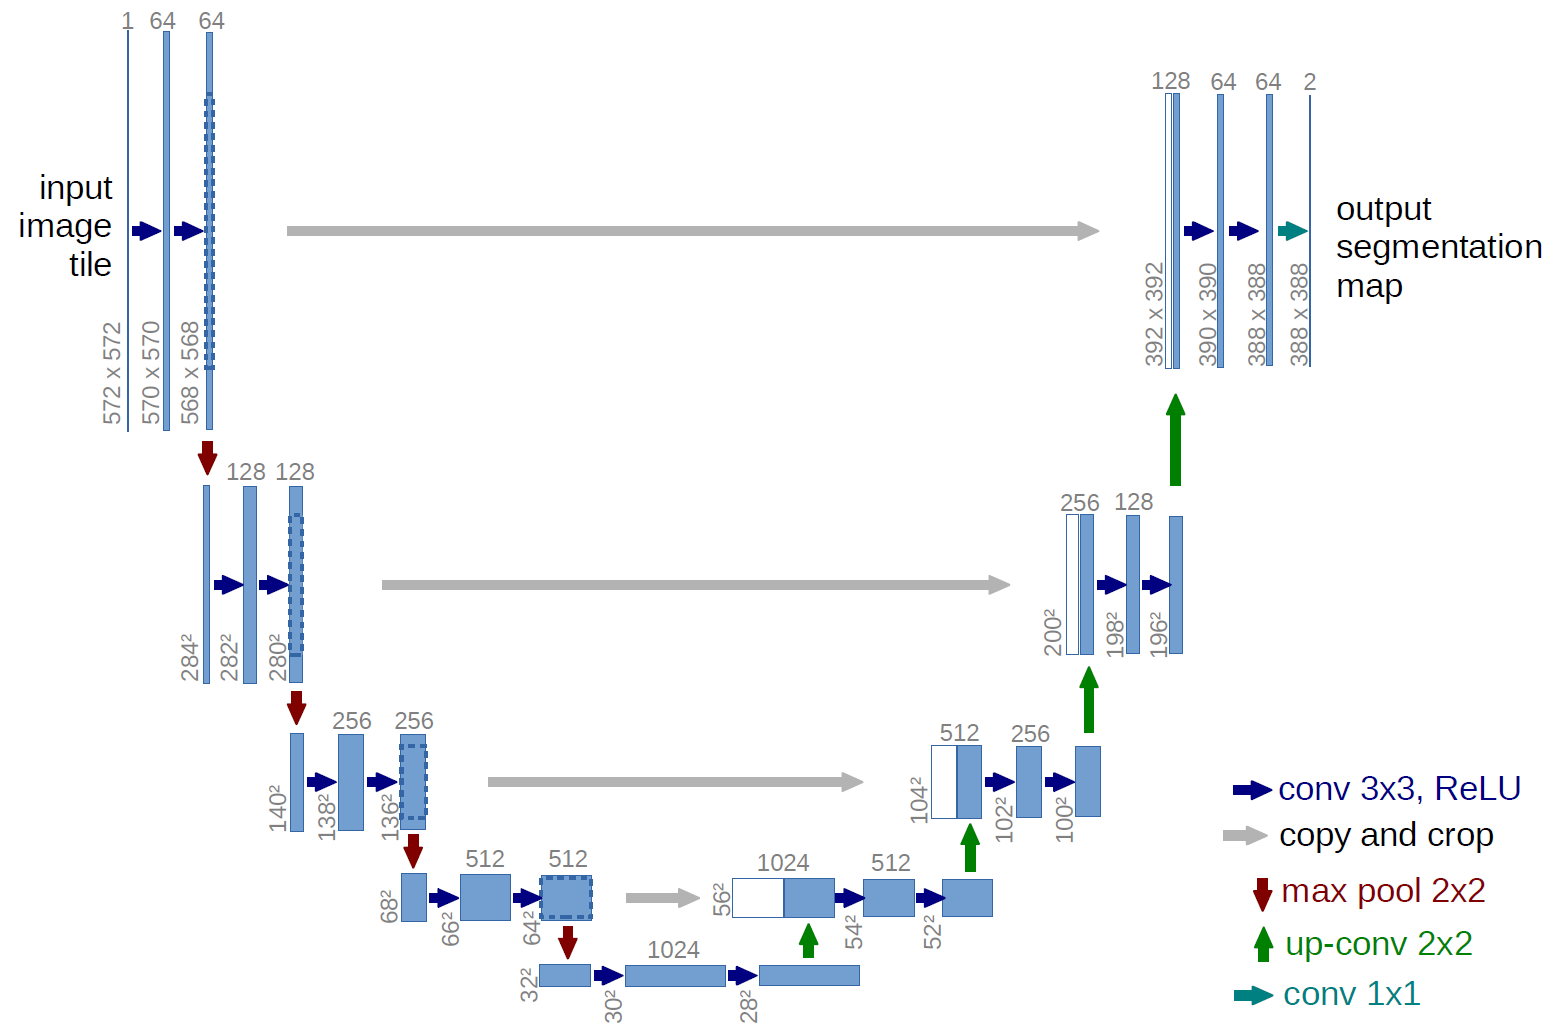
\includegraphics[width=.4\textwidth]{Imgs/u-net-architecture.png}
        \caption{Arquitectura de una U-net.}
        \label{fig:u-net}
    \end{figure}

    El error del generador es cuantizado por la red discriminativa.

    \subsubsection{Discriminador}

    El discriminador posee una arquitectura mucho mas sencilla, la cual consta de $6$ capas de convolución.
    Esto se debe a que la salida representa que tan realista es un segmento de la imagen de entrada. 
    El error del discriminador se cuantiza mediante una entropía cruzada. Ya que 
    se propone que siempre que le entre una imagen del generador la salida debe ser una matriz de $0$, ya que 
    esta imagen no es del dataset, mientras que cuando la entrada sea una imagen del dataset el resultado debe ser un $1$. 
    
    Estodesemboca en una pelea entre en generador ya que debe aprender a engañar al discriminador 
    y el discriminador que debe lograr siempre reconocer que la imagen $\hat{Y}$ es totalmente falsa, ya que es una 
    creación de la red generativa.
 
    \subsection{Preporcesado de los datos}

    Un paso fundamental para trabajar con algoritmos de imagenes es pasar del domininio $[0;255]$ a 
    un dominio mas acotado, para este trabajo se utilizo el domino de $[-1;1]$. De esta forma se logra 
    una mayor eficiencia computacional.

    Debido al tamaño de las imagenes es recomendable hacer un resize a dimensiones mas pequeñas 
    para disminuir el uso de RAM cuando son cargadas en memoria y el uso de GPU al realizar las convoluciones. En 
    este caso las imagenes de entrada y de salida son redimensionadas a $256x256$.

    \subsubsection{Random jitter}

    El \textit{random jitter} es un proceso por en el cual se busca realizar un aumentado
    del dataset, esto disminuye la posibilidad de experimentar \textbf{overfitting}. 
    Este proceso cuenta de $2$ pasos:

    \begin{itemize}
        \item[Crop] Se realiza un resize a $286x286$ para luego realizar un recorte a $25x256$.
        \item[Flip] De forma aletoria con probabilidad $0.5$ se realiza un rotación de $180^\circ$. 
    \end{itemize}

    Debido a que es utiliza en algoritmos supervisados es necesario aplicar 
    el \textit{random jitter} tanto a la imagen de entrada como a la de salida,
    para ello se hace un stack de las mismas como se observa en la Fig.\ref{fig:random-jitter}.

    \begin{figure}
        \centering
        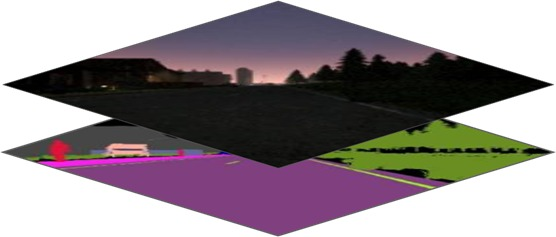
\includegraphics[width=.4\textwidth]{Imgs/stack-random-jitter.jpeg}
        \caption{Visualización del stack previo al random jitter.}
        \label{fig:random-jitter}
    \end{figure}

    En la Fig.\ref{fig:crop-flip} se observa el proceso de random jitter completo.

    \begin{figure}
        \centering
        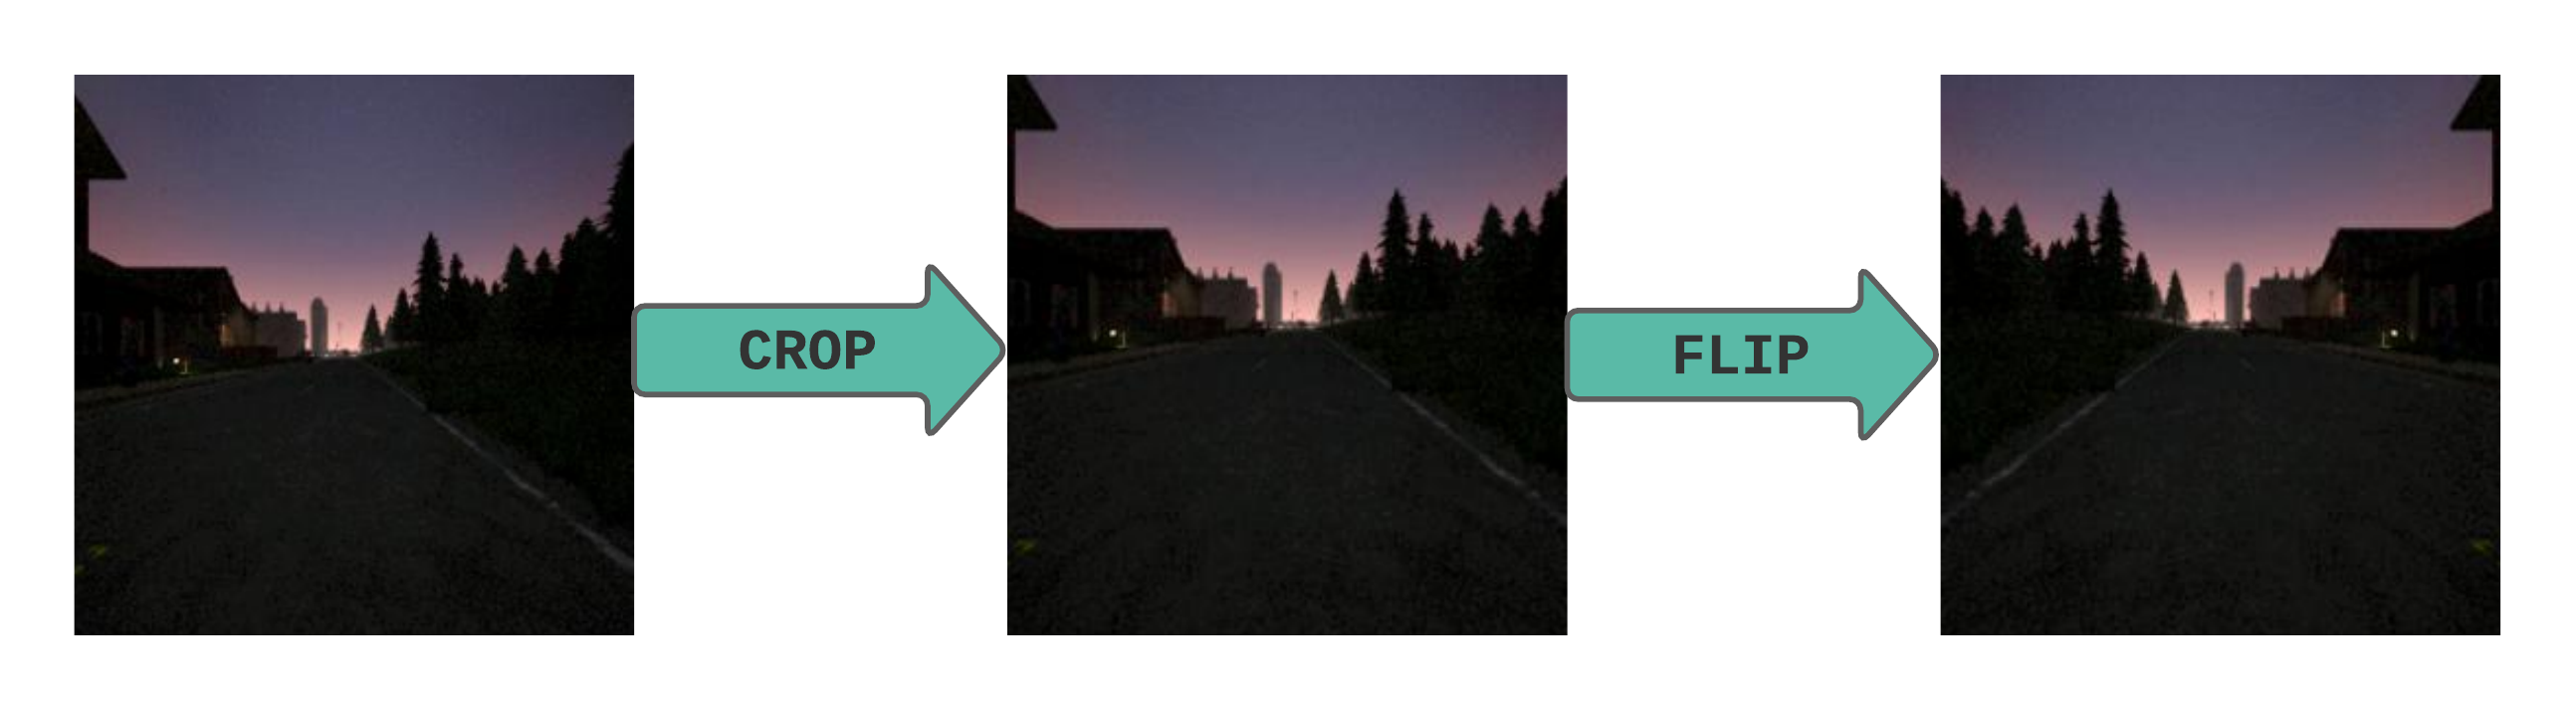
\includegraphics[width=.4\textwidth]{Imgs/in_crop_flip.png}
        \caption{Visualización del random jitter.}
        \label{fig:crop-flip}
    \end{figure}

    \section{Desarrollo}

    Se presentara de forma ordena todas las etapas del proyecto. 
    Debido a la cantidad de imagenes utilizadas no es posible presentarlas a todas, por ello 
    se relizaran analisís particulares para algunos casos de interes.

    \subsection{Obtención del dataset}

    Para obtener el dataset se colocaron una camara RGB y una camara de segmentación semántica
    \cite{CARLA-Sensors-Reference}, ubicadas en la misma posición. Se recolectaron los datos 
    cada 5 segundos. Las condiciones climaticas utilizadas fueron aletorias, lo que permite 
    obtener un dataset mucho mas variado Fig.\ref{fig:dataset}.

    \begin{figure}
        \centering
        %\includegraphics[width=.5\textwidth]{Imgs/tar_crop.jpg}
        \caption{Imagenes de muestra del dataset}
        \label{fig:dataset}
    \end{figure}

    Para lograr un manejo autónomo del vehículo se utilizó el autopilot \cite{CARLA-Documentation}. 
    Con la finalidad de aumentar la variedad de imágenes se utilizaron todos los mapas posibles y 
    se adicionaron otros vehiculos autónomos junto a personas. Aunque debido 
    a limitaciones de hardware solo se pudieron ingresar 20 personas, lo cual 
    provocó una deficiencia en la detección de personas de la red Pix2Pix. 

    \subsection{Entrenamiento de la red}

    Como fue mencinado en el marco teoríco el modelo implementado se denomina Pix2Pix \cite{Pix2Pix}.
    Se utilizó como entrada la imagen de la camara RGB y la salida será una imagen segmentada, para ello se utilizó
    el dataset obtenido con el simulador de \textbf{CARLA} el cual posee 8000 imagenes. 

    \subsubsection{Tratamiento de las imagenes}

    Para evitar problemas en el entrenamiento de la red es muy usual llevar los valores de cada canal al 
    intervalor $[-1;1]$, esto evita problemas de continuidad en red. Luego 
    se procede a aplicar un \textit{random jitter}.

    El dataset fue dividido en 2 partes una utilizada para el entrenamiento, aproximadamente el $80 \% $ de las imagenes y 
    otra parte para el testing de la red utilizando el $20 \%$ restante, siguiendo el principio de Pareto.

    \subsubsection{Entrenamiento}

    Para realizar el entremiento se utlizó el dataset de testin, aproximadamente 6400 imagenes, 
    y se realizon 400 iteración a la red para lograr un mejor desenpeñó. 
    
    En la Fig.\ref{fig:resultados}
    se muestra una comparación para $1$ imagen del dataset de testing luego de la primera iteración 
    y al finalizar el entrenamiento.
    Puede observarse que existieron grandes mejoras sobre todo en la zona de la palmera
    donde al finalizar el entrenamiento es posible observar los detalles de la misma.
    Aunque cabe destacar que debido a la poca cantidad de señales de trafico en el dataset
    se observa que si bien reconoce la estructura del semaforo no es capaz de utilizar el color 
    adecuado.

    \begin{figure}[htb]
        \centering
        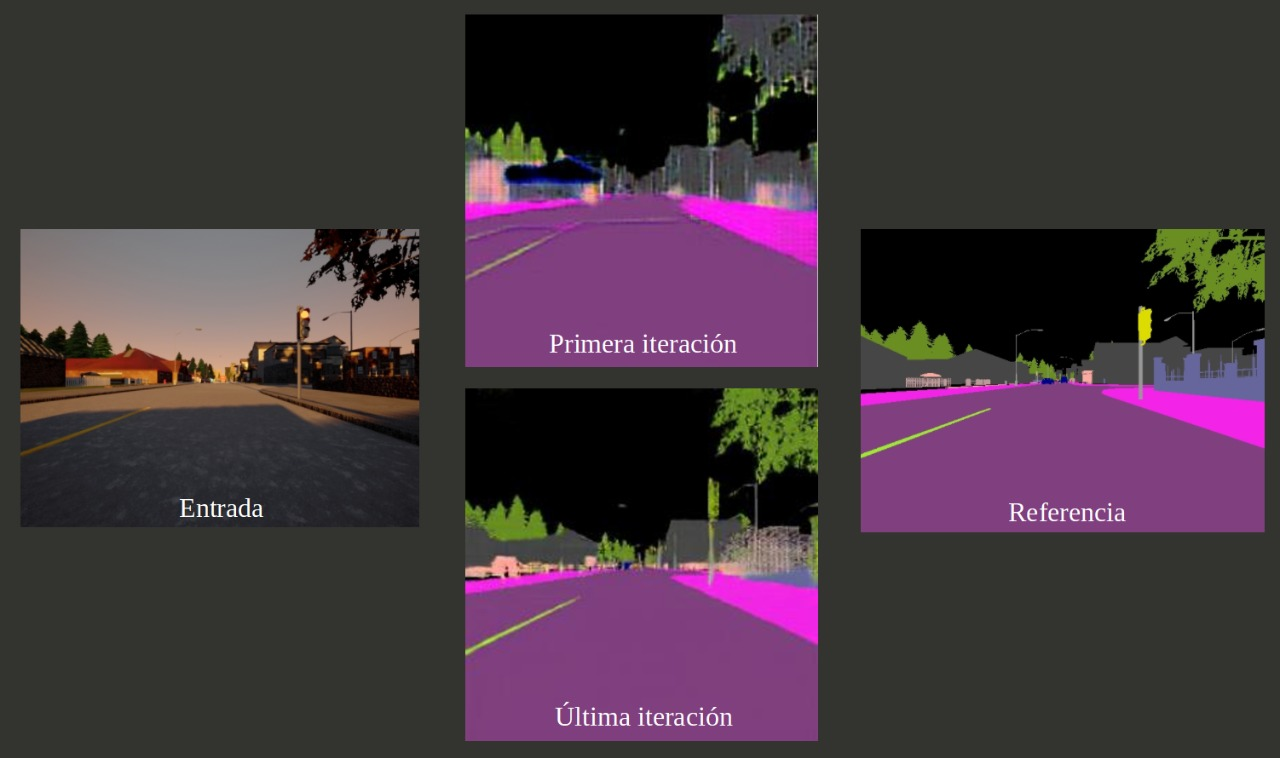
\includegraphics[width=.4\textwidth]{Imgs/grapics_results.jpg}    
        \caption{Imagen del dataset de testing.}
        \label{fig:resultados}
    \end{figure}

    Al analizar otro imagen del dataset la cual se observa en la Fig.\ref{fig:person_image}
    {COMPLETAR!!!}



    \section{Resultados}
    En esta sección se veran los resultados obtenidos tanto para imágenes del simulador como para imágenes reales. Además se dejará un 
    link de un video demostrativo.
    \subsection{Imágenes del simulador}


    \subsection{Imágenes reales}




    \section{Conclusiones}
    Observando la \ref{fig:resultados2} se puede concluir que los resultados son bastante precisos si lo comparamos con la
    imagen semántica del simulador. Si bien ciertos detalles como las paradas de colectivo, señales de transito o peatones no los 
    reconoce o si lo hace no le asiga el color adecuado, en las regiones mas significativas como los autos, la calle o la vereda 
    logra un desempeño bastante aceptable. Por otro lado, en la \ref{fig:resulReales} donde se analiza a la red con imágenes reales,
    se observa que existen mas errores a la hora de segmentar. Hay regiones que no se delimitan correctamente y/o colores que no son 
    los adecuados. Por ejemplo la mancha azul en los arbustos de la primera imágen. Las regiones mas significativas en este caso logran un 
    resultado semi aceptable que aun asi se podrian utilizar para darle redundancia al sistema autónomo. Lo más probable es que estos 
    errores se deban a la diferencia de iluminación y la cantidad de detalles que tiene una imagen real en comparación con las imagenes 
    de CARLA.
    \subsubsection{Ventajas}
    A continuación se nombraran algunas ventajas de realizar la segmentación semántica, en particular con un simulador y una red Pix2Pix:
    \begin{enumerate}
        \item La ventaja principal que tiene segmentar semánticamente una imagen es la posibilidad de reconocer objetos o zonas de una forma
        mucho mas sencilla ya sea para un usuario o para un software. Una ventaja secundaria de las imágenes semánticas es que ocupan menos espacio 
        en memoria que su equivalente en RGB.
        \item Al utilizar un simulador la principal ventaja recae en la posibilidad de crear un dataset con el mínimo esfuerzo humano, tiempo y costo monetario.
        Por otro lado, a la hora de recolectar información el simulador permite una gran flexibilidad de simular situaciones externas o propias del
        vehículo. Poder variar el clima, el mapa, la velocidad del auto de prueba o los de la ciudad, entre otras muchas características. Esto nos permite 
        simular situaciones anómalas y asi crear un dataset mucho mas variado. 
        \item La implementación de una red Pix2Pix para realizar la segmentación semántica tiene como principal ventaja....
    \end{enumerate}
    \subsubsection{Desventajas}
    Teniendo en cuenta las ventajas mencionadas anteriormente, veremos las desventajas o inconvenientes:
    \begin{itemize}
        \item La principal desventaja de utilizar un simulador para esta tarea es la diferencia que se presenta entre el entorno simulado y el real.
        Como quedó envidenciado en los resultados, esta diferencia de entornos genera errores en la imagen final. Por otro lado, se necesitarian 
        conocimientos de programación en simuladores para generar un entornos mucho mas reales o con características particulares. 
        \item A la hora de implementar la red neuronal las desventajas recaen en la cantidad de tiempo necesario para entrenarlas, el costo computacional 
        y en particular ... %Poner eso de que no se puede editar mucho, como si fuera un sistema cerrado
        Además, a la hora de entrenar a la red es necesario en la mayoria de los casos un dataset de gran tamaño y heterogéneo. 
    \end{itemize}


    Por último, como conclusión general cabe destacar que este tipo de prácticas son muy importantes y utilizadas en la actualidad. Las redes neuronales 
    estan revolucionando la forma de trabajar y pensar en distos ámbitos. En consencuencia, existen grandes costos tanto monetarios como temporales que provocan el generar un
    dataset. Debido a esto, el implementar un simulador que disminuya estos factores limitantes es una de las técnicas bien vistas al día de hoy.


    \bibliographystyle{IEEEannot}
    \bibliography{biblio}
\end{document}